\documentclass{article}
\usepackage{algpseudocodex}
\usepackage{algorithmicx}
\usepackage{enumitem}
\usepackage[boxed]{algorithm}
\usepackage{float}
\usepackage[utf8]{inputenc}
\usepackage{amsmath}
\usepackage{amssymb}
\usepackage{graphicx}
\usepackage{subfig}
\usepackage{tcolorbox}
\usepackage{listings}
\usepackage[left=20mm, right=20mm]{geometry}
\usepackage{enumitem}
\usepackage{amsthm}
\usepackage{algpseudocodex}
\usepackage{algorithmicx}
\usepackage[boxed]{algorithm}
\usepackage{hyperref}
\usepackage{tikz}
\usepackage{xcolor}
\usepackage{colortbl} % For coloring cells and text
\usepackage{amsmath}  % For mathematical symbols
\usepackage{forest}
\usetikzlibrary{shapes.geometric, arrows.meta, positioning, calc}

\newtheorem{theorem}{Theorem}
\newtheorem{lemma}{Lemma}
\newtheorem{corollary}{Corollary}[theorem]
\newtheorem{corollaryLemma}{Corollary}[lemma]
\newtheorem{prop}{Proposition}
\newtheorem{claim}{Claim}[theorem]

\definecolor{dupcolor}{RGB}{255,0,0} % Red
\definecolor{maxintcolor}{RGB}{165,42,42} % Brown
\definecolor{subsetsumcolor}{RGB}{0,0,255} % Blue

\lstset{showstringspaces=false,
        numbers=left, 
		numberstyle=\small}
\graphicspath{{}}

\algdef{SE}[CLASS]{Class}{EndClass}[1]{\textbf{Class} \textsc{#1}}{}
\algnewcommand{\AND}{\textbf{ and }}
\algnewcommand{\OR}{\textbf{ or }}
\algnewcommand{\Int}{\textbf{int }}
\algnewcommand{\Real}{\textbf{real }}

\title{COMP2123-Assignment 5}

\begin{document}
	\maketitle
	\section*{Notation Clarification}
	This section is to clarify the notations used throughout this assignment.
	
	\begin{center}
		\begin{tabular}{ c c }
			\([a:b]\) & The sequence \(a,\, a + 1, \ldots, \, b - 1\).\\
			\verb|int| & The data type representing integers.\\
			\verb|real| & The data type representing the real numbers.\\
			\verb|void| & Used to show that a function does not return anything.\\
			\verb|null| & The variable representing nothingness.\\
			\verb|bool| & The data type representing a boolean value which is either true or false.\\
			\verb|!| & Logical expressions and performing logical negation in programming\\

		\end{tabular}
	\end{center} 

	\newpage \section*{Problem 1: Recurrence Relations Analysis}
	\subsection*{a) \(T(n) = 3T(n/2) + n^2\)}
	\begin{tikzpicture}
		\node (Tn) at (0,0) {$T(n)$};
		\node (Tn2-1) at (-3,-1.5) {$T\left(\frac{n}{2}\right)$};
		\node (Tn2-2) at (0,-1.5) {$T\left(\frac{n}{2}\right)$};
		\node (Tn2-3) at (3,-1.5) {$T\left(\frac{n}{2}\right)$};
		\node (Tn4-1) at (-7,-3) {$T\left(\frac{n}{2^2}\right)$};
		\node (Tn4-2) at (-5,-3) {$T\left(\frac{n}{2^2}\right)$};
		\node (Tn4-3) at (-3,-3) {$T\left(\frac{n}{2^2}\right)$};
		
		\draw (Tn) -- (Tn2-1);
		\draw (Tn) -- (Tn2-2);
		\draw (Tn) -- (Tn2-3);
		\draw (Tn2-1) -- (Tn4-1);
		\draw (Tn2-1) -- (Tn4-2);
		\draw (Tn2-1) -- (Tn4-3);
		\draw (Tn2-2) -- (-2, -3);
		\draw (Tn2-2) -- (-1, -3);
		\draw (Tn2-2) -- (0, -3);
		\draw (Tn2-3) -- (1, -3);
		\draw (Tn2-3) -- (2, -3);
		\draw (Tn2-3) -- (3, -3);
		
		% Cost Function Annotations
		\node at (5,0) {$cn^2$};
		\node at (5,-1.5) {$3c\left(\frac{n}{2}\right)^2$};
		\node at (5,-3) {$3^2c\left(\frac{n}{2^2}\right)^2$};
		\node at (5,-4.5) {$3^k c\left(\frac{n}{2^k}\right)^2$};
		
		% Levels
		\draw[dotted] (-8,0) -- (11,0);
		\draw[dotted] (-8,-1.5) -- (11,-1.5);
		\draw[dotted] (-8,-3) -- (11,-3);
		\draw[dotted] (-8,-4.5) -- (11,-4.5);
		
		\node at (-9,0) {level 0};
		\node at (-9,-1.5) {level 1};
		\node at (-9,-3) {level 2};
		\node at (-9,-4.5) {level $k$};
	  \end{tikzpicture}
	  \begin{itemize}
		\item Since we halve the size every time, there are totally \( k = \log_{2}n \) levels. Summing all this up, we get:
		\begin{align}
			T(n) &= cn^2 + 3c\left(\frac{n}{2}\right)^2 + 3^2c\left(\frac{n}{2^2}\right)^2 + 3^3c\left(\frac{n}{2^3}\right)^2 + \ldots + 3^kc\left(\frac{n}{2^k}\right)^2 \label{eq:initial_sum} \\
				 &=  cn^2 \left( 3^0 \left(\frac{1}{2^0}\right)^2 + 3^1 \left(\frac{1}{2}\right)^2 +  3^2 \left(\frac{1}{2^2}\right)^2 + 3^3 \left(\frac{1}{2^3}\right)^2 + ... + 3^k \left(\frac{1}{2^k}\right)^2 \right) \\
				 &=  cn^2 \left( 3^0 \left(\frac{1}{2^2}\right)^0 + 3 \left(\frac{1}{2^2}\right) +  3^2 \left(\frac{1}{2^2}\right)^2 + 3^3 \left(\frac{1}{2^2}\right)^3 + ... + 3^k \left(\frac{1}{2^2}\right)^k \right) \\
				 &=  cn^2 \left( 1 + \left(\frac{3}{4}\right) +  \left(\frac{3}{4}\right)^2 + \left(\frac{3}{4}\right)^3 + \ldots + \left(\frac{3}{4}\right)^k \right) \\
				 &= cn^2 \left( \sum_{i = 0}^{\log_{2}n} \left(\frac{3}{4}\right)^i \right) \label{1:a:1}
		\end{align}
		\item When we apply the bound on the geometric series to \eqref{1:a:1} with \( r = \frac{3}{4} \), we get:
		\begin{align}
			T(n) &= cn^2 \left( \frac{1 - \left(\frac{3}{4}\right)^{\log_2n + 1}}{1 - \frac{3}{4}} \right) \\
				 &= cn^2 \left( 4 \left( 1 - \left(\frac{3}{4}\right)^{\log_2n + 1} \right) \right) \\
				 &= cn^2 \left( 4 - 4 \cdot \frac{3}{4} \cdot \left(\frac{3}{4}\right)^{\log_2n} \right) \\
				 &=  cn^2 \left( 4 - 3 \cdot \left(\frac{3}{4}\right)^{\log_2n} \right) 
		\end{align}
		\item Using the formula \(a^{\log_2b} = b^{\log_2a} \), we have:
		\begin{align*}
			T(n) &=  cn^2 \left( 4 - 3 \cdot \left(n\right)^{\log_2\frac{3}{4}} \right) \\
				 &= cn^2 \left( 4 - 3 \cdot \left(n\right)^{\log_2 3 - 2} \right) \\
				 &= cn^2 \left( 4 - 3 \cdot \left(\frac{n^{\log_2 3}}{n^2}\right) \right) \\
				 &= 4cn^2 - 3cn^2 \cdot \frac{n^{\log_2 3}}{n^2} \\
				 &= 4cn^2 - 3cn^{\log_2 3} \\
		\end{align*}
	\end{itemize}
	Since \(\log_2 3\) is a constant, the term \(3cn^{\log_2 3}\) is much smaller than \(4cn^2\) as \(n\) grows larger. Therefore, the dominant term is \(4cn^2\), and we can conclude that \(T(n) = \Theta(n^2)\).

	\subsection*{b) \(T(n) = 4T(n/2) + n\)}
	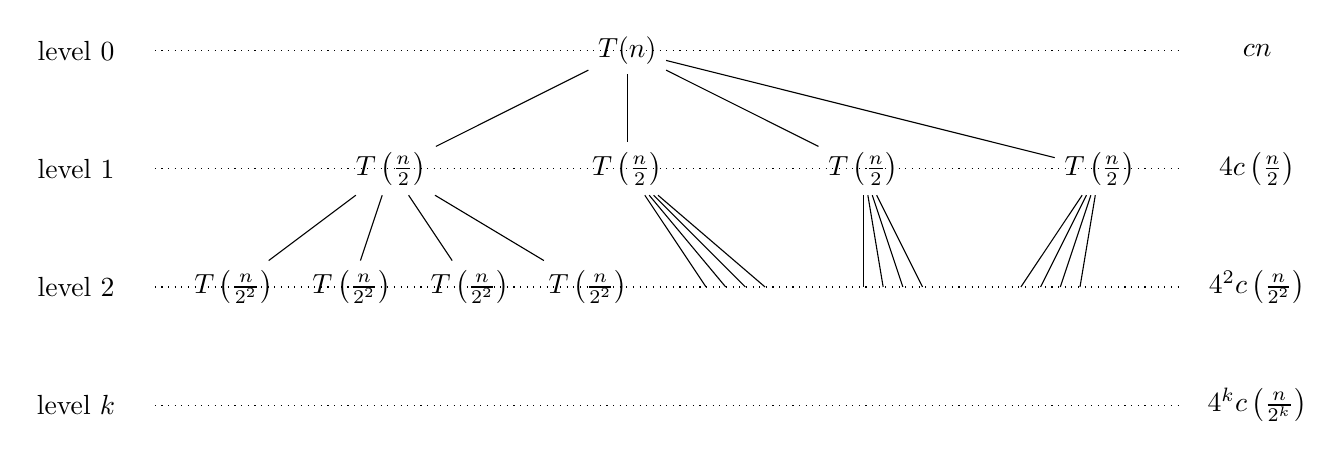
\begin{tikzpicture}
		\node (Tn) at (0,0) {$T(n)$};
		\node (Tn2-1) at (-3,-1.5) {$T\left(\frac{n}{2}\right)$};
		\node (Tn2-2) at (0,-1.5) {$T\left(\frac{n}{2}\right)$};
		\node (Tn2-3) at (3,-1.5) {$T\left(\frac{n}{2}\right)$};
		\node (Tn2-4) at (6, -1.5) {$T\left(\frac{n}{2}\right)$};
		\node (Tn4-1) at (-5,-3) {$T\left(\frac{n}{2^2}\right)$};
		\node (Tn4-2) at (-3.5,-3) {$T\left(\frac{n}{2^2}\right)$};
		\node (Tn4-3) at (-2,-3) {$T\left(\frac{n}{2^2}\right)$};
		\node (Tn4-4) at (-0.5,-3) {$T\left(\frac{n}{2^2}\right)$};
		
		\draw (Tn) -- (Tn2-1);
		\draw (Tn) -- (Tn2-2);
		\draw (Tn) -- (Tn2-3);
		\draw (Tn) -- (Tn2-4);
		\draw (Tn2-1) -- (Tn4-1);
		\draw (Tn2-1) -- (Tn4-2);
		\draw (Tn2-1) -- (Tn4-3);
		\draw (Tn2-1) -- (Tn4-4);
		\draw (Tn2-2) -- (1, -3);
		\draw (Tn2-2) -- (1.25, -3);
		\draw (Tn2-2) -- (1.5, -3);
		\draw (Tn2-2) -- (1.75, -3);
		\draw (Tn2-3) -- (3, -3);
		\draw (Tn2-3) -- (3.25, -3);
		\draw (Tn2-3) -- (3.5, -3);
		\draw (Tn2-3) -- (3.75, -3);
		\draw (Tn2-4) -- (5, -3);
		\draw (Tn2-4) -- (5.25, -3);
		\draw (Tn2-4) -- (5.5, -3);
		\draw (Tn2-4) -- (5.75, -3);

		
		% Cost Function Annotations
		\node at (8,0) {$cn$};
		\node at (8,-1.5) {$4c\left(\frac{n}{2}\right)$};
		\node at (8,-3) {$4^2c\left(\frac{n}{2^2}\right)$};
		\node at (8,-4.5) {$4^kc\left(\frac{n}{2^k}\right)$};
		
		% Levels
		\draw[dotted] (-6,0) -- (7,0);
		\draw[dotted] (-6,-1.5) -- (7,-1.5);
		\draw[dotted] (-6,-3) -- (7,-3);
		\draw[dotted] (-6,-4.5) -- (7,-4.5);
		
		\node at (-7,0) {level 0};
		\node at (-7,-1.5) {level 1};
		\node at (-7,-3) {level 2};
		\node at (-7,-4.5) {level $k$};
	\end{tikzpicture}
	\begin{itemize}
		\item Since we halve the size every time, there are totally \( k = \log_{2}n \) levels. Summing all this up, we get:
		\begin{align}
			T(n) &= cn + 4c\left(\frac{n}{2}\right) + 4^2c\left(\frac{n}{2^2}\right) + 4^3c\left(\frac{n}{2^3}\right) + \ldots + 4^kc\left(\frac{n}{2^k}\right) \\
			     &= cn\left(\left(\frac{4}{2}\right)^0 + \left(\frac{4}{2}\right)^1+ \left(\frac{4}{2}\right)^2 + \left(\frac{4}{2}\right)^3 + ... + \left(\frac{4}{2}\right)^k \right)\\ 
				 &= cn(1 + 2 + 2^2 + 2^3 + ... + 2^k) \label{1:b:1}
		\end{align}
		\item When we apply the bound on the geometric series to \eqref{1:b:1} with \( r = 2 \), we get:
		\begin{align}
			T(n) &= cn(\frac{1 - 2^{k + 1}}{1 - 2})\\
			     &= cn(2^{k + 1} - 1) \\
				 &= cn\left(2\cdot2^k - 1\right) \\
				 &= 2cn\cdot2^{log_2n} - cn \\
		\end{align}
		\item Using the formula \( a^{\log_2b} = b^{\log_2a} \), we have:
		\begin{align}
			T(n) &= 2cn\cdot n^{log_22} - cn \\
				 &= 2cn^2 - cn
		\end{align}
		the term \(cn\) is much smaller than \(2cn^2\) as \(n\) grows larger. Therefore, the dominant term is \(2cn^2\), and we can conclude that \(T(n) = \Theta(n^2)\).
	\end{itemize}

	\subsection*{c) \(T(n) = T(n - 1) + n\)}
	\begin{tikzpicture}
		\node (Tn) at (0,0) {$T(n)$};
		\node (Tn2-1) at (0,-1.5) {$T\left(n - 1\right)$};
		\node (Tn4-1) at (0,-3) {$T\left(n - 2\right)$};
		
		\draw (Tn) -- (Tn2-1);
		\draw (Tn2-1) -- (Tn4-1);

		
		% Cost Function Annotations
		\node at (8,0) {$cn$};
		\node at (8,-1.5) {$c\left(n - 1\right)$};
		\node at (8,-3) {$c\left(n - 2\right)$};
		\node at (8,-4.5) {$c\left(n - k\right)$};
		
		% Levels
		\draw[dotted] (-6,0) -- (7,0);
		\draw[dotted] (-6,-1.5) -- (7,-1.5);
		\draw[dotted] (-6,-3) -- (7,-3);
		\draw[dotted] (-6,-4.5) -- (7,-4.5);
		
		\node at (-7,0) {level 0};
		\node at (-7,-1.5) {level 1};
		\node at (-7,-3) {level 2};
		\node at (-7,-4.5) {level $k$};
	\end{tikzpicture}
	\begin{itemize}
		\item Since we reduce the size by 1 every time, there are totally \( k = n - 1\) levels. Summing all this up, we get:
		\begin{align}
			T(n) &= cn + c(n - 1) + c(n - 2) + c(n - 3) + ... + c(n - k) \\
				 &= c(n + (n - 1) + ... + 3 + 2 + 1) \label{1:c:1}
		\end{align}
		\item We have formula \(1 + 2 + 3 + ... + n = \frac{n(n + 1)}{2} for\) \eqref{1:c:1}, we have:
		\begin{align*}
			T(n) &= c\frac{n(n + 1)}{2} \\
                 &= \frac{c}{2}n^2 + \frac{c}{2}n\\
		\end{align*}
		The term \(\frac{1}{2}cn\) is much smaller than \(\frac{1}{2}cn^2\) as \(n\) grows larger. Therefore, the dominant term is \(\frac{1}{2}cn^2\), and we can conclude that \(T(n) = \Theta(n^2)\).
	\end{itemize}

	\subsection*{d) \(T(n) = 2T(n/2) + n \log n\)}
	\begin{tikzpicture}
		\node (Tn) at (0,0) {$T(n)$};
		\node (Tn2-1) at (-3,-1.5) {$T\left(\frac{n}{2}\right)$};
		\node (Tn2-2) at (3,-1.5) {$T\left(\frac{n}{2}\right)$};
		\node (Tn4-1) at (-5,-3) {$T\left(\frac{n}{2^2}\right)$};
		\node (Tn4-2) at (0,-3) {$T\left(\frac{n}{2^2}\right)$};
		
		\draw (Tn) -- (Tn2-1);
		\draw (Tn) -- (Tn2-2);
		\draw (Tn2-1) -- (Tn4-1);
		\draw (Tn2-1) -- (Tn4-2);
		\draw (Tn2-2) -- (3, -3);
		\draw (Tn2-2) -- (6, -3);


		
		% Cost Function Annotations
		\node at (8,0) {$c\cdot n \cdot \log_2n$};
		\node at (8,-1.5) {$2c\cdot \frac{n}{2} \cdot \log_2(\frac{n}{2})$};
		\node at (8,-3) {$2^2c\cdot \frac{n}{2^2} \cdot \log_2(\frac{n}{2^2})$};
		\node at (8,-4.5) {$2^kc\cdot \frac{n}{2^k} \cdot \log_2(\frac{n}{2^k})$};
		
		% Levels
		\draw[dotted] (-6,0) -- (7,0);
		\draw[dotted] (-6,-1.5) -- (7,-1.5);
		\draw[dotted] (-6,-3) -- (7,-3);
		\draw[dotted] (-6,-4.5) -- (7,-4.5);
		
		\node at (-7,0) {level 0};
		\node at (-7,-1.5) {level 1};
		\node at (-7,-3) {level 2};
		\node at (-7,-4.5) {level $k$};
	\end{tikzpicture}

	\begin{itemize}
		\item Since we halve the size every time, there are totally \( k = \log_{2}n \) levels. Summing all this up, we get:
		\begin{align}
			T(n) &= cn \cdot \log_2n + 2c\cdot \frac{n}{2} \cdot \log_2(\frac{n}{2}) + 2^2c\cdot \frac{n}{2^2} \cdot \log_2(\frac{n}{2^2}) + ... + 2^kc\cdot \frac{n}{2^k} \cdot \log_2(\frac{n}{2^k})\\\
			     &= cn\left(log_2n + 2\frac{1}{2}\log_2(\frac{n}{2}) + 2^2\frac{1}{2^2}\log_2(\frac{n}{2^2}) +... + 2^k\frac{1}{2^k} \log_2(\frac{1}{2^k})\right) \\
				 &= cn\left(log_2n + log_2(\frac{n}{2}) + log_2(\frac{n}{2^2}) + ... + log_2(\frac{n}{2^k})\right) \\
				 &= cn\left((log_2n - log_22^0)+ (log_2n - log_22) + (log_2n - log_22^2) ... + (log_2n - log_22^k)\right) \\
				 &= cn\left((k + 1)log_2n - (log_22^0 + log_22^1 + log_22^2 + ... + log_22^k)\right) \\
				 &= cn\left(klog_2n + log_2n - (0log_22 + 1log_22 + 2 log_2^2 + ... + klog_22 )\right) \Comment{Using Power rule of logarithms} \\
				 &= cn\left(klog_2n + log_2n - (0 + 1 + 2 + ... k)\right) \\
				 &= cn\left(klog_2n + log_2n - \frac{k(k + 1)}{2}\right) \\
				 &= cn\left((log_2n)^2 + log_2n - \frac{log_2n(log_2n + 1)}{2}\right) \\
				 &= cn\left((log_2n)^2 + log_2n - \frac{(log_2n)^2 + log_2n}{2}\right) \\
				 &= cn(log_2n)^2 + cnlog_2n - \frac{1}{2}cn(log_2n)^2 - \frac{1}{2}cn(log_2n)\\
				 &= \frac{1}{2}cn(log2_n)^2 -  \frac{1}{2}cn(log_2n) \\
		\end{align}
	\end{itemize}
	The term \(\frac{1}{2}cn(log_2n)\) is much smaller than \(\frac{1}{2}cn(log2_n)^2\) as \(n\) grows larger. Therefore, the dominant term is \(\frac{1}{2}cn^2\), and we can conclude that \(T(n) = \Theta(n(log_2n)^2)\).

	\subsection*{e) \(T(n) = \sqrt{2}T(n/2) + \log n\)}

	In this case, we have:
	\[n^{\log_b{a}} \text{ is } n^{\log_2\sqrt{2}} \text{ which is } n^{1/2}\]
	And we also have, \(f(n) = \log_2n\). Since \(\log_2n\) is asymptotically less than any positive number of n \(f(n)\) is \((n^{\log_ba - \epsilon})\) for any \(0 < \epsilon < \frac{1}{2}\). Therefore, by Master Theorem, \(T(n)\) is \(\Theta(\sqrt{n})\) in this case
	

	\subsection*{f) \(T(n) = 3T(n/3) + \sqrt{n}\)}
	\begin{tikzpicture}
		\node (Tn) at (0,0) {$T(n)$};
		\node (Tn2-1) at (-3,-1.5) {$T\left(\frac{n}{3}\right)$};
		\node (Tn2-2) at (0,-1.5) {$T\left(\frac{n}{3}\right)$};
		\node (Tn2-3) at (3,-1.5) {$T\left(\frac{n}{3}\right)$};
		\node (Tn4-1) at (-7,-3) {$T\left(\frac{n}{3^2}\right)$};
		\node (Tn4-2) at (-5,-3) {$T\left(\frac{n}{3^2}\right)$};
		\node (Tn4-3) at (-3,-3) {$T\left(\frac{n}{3^2}\right)$};
		
		\draw (Tn) -- (Tn2-1);
		\draw (Tn) -- (Tn2-2);
		\draw (Tn) -- (Tn2-3);
		\draw (Tn2-1) -- (Tn4-1);
		\draw (Tn2-1) -- (Tn4-2);
		\draw (Tn2-1) -- (Tn4-3);
		\draw (Tn2-2) -- (-2, -3);
		\draw (Tn2-2) -- (-1, -3);
		\draw (Tn2-2) -- (0, -3);
		\draw (Tn2-3) -- (1, -3);
		\draw (Tn2-3) -- (2, -3);
		\draw (Tn2-3) -- (3, -3);
		
		% Cost Function Annotations
		\node at (5,0) {$c\sqrt{n}$};
		\node at (5,-1.5) {$3c\sqrt{\frac{n}{3}}$};
		\node at (5,-3) {$3^2c\sqrt{\frac{n}{3^2}}$};
		\node at (5,-4.5) {$3^kc\sqrt{\frac{n}{3^k}}$};
		
		% Levels
		\draw[dotted] (-8,0) -- (11,0);
		\draw[dotted] (-8,-1.5) -- (11,-1.5);
		\draw[dotted] (-8,-3) -- (11,-3);
		\draw[dotted] (-8,-4.5) -- (11,-4.5);
		
		\node at (-9,0) {level 0};
		\node at (-9,-1.5) {level 1};
		\node at (-9,-3) {level 2};
		\node at (-9,-4.5) {level $k$};
	  \end{tikzpicture}
	\begin{itemize}
		\item Since we reduce the size by a factor of three each time, there are totally \( k = \log_3n\) levels. Summing all this up, we get:'
		\begin{align}
			T(n) &= c\sqrt{n} + 3c\sqrt{\frac{n}{3}} + 3^2c\sqrt{\frac{n}{3^2}} + ... + 3^kc\sqrt{\frac{n}{3^k}} \\
			    &= c\sqrt{n}\left(3^0 \sqrt{\frac{1}{3^0}} + 3^1 \sqrt{\frac{1}{3^1}} + 3^2 \sqrt{\frac{1}{3^2}} + ... + 3^k \sqrt{\frac{1}{3^k}}\right) \\
				&= c\sqrt{n}\left(\sqrt{\frac{(3^0)^2}{3^0}} + \sqrt{\frac{(3^1)^2}{3^1}} + \sqrt{\frac{(3^2)^2}{3^2}} + ... + \sqrt{\frac{(3^k)^2}{3^k}}\right) \\
				&= c\sqrt{n}\left(\sqrt{3^0} + \sqrt{3^1} + \sqrt{3^2} + ... + \sqrt{3^k}\right) \\
				&= c\sqrt{n}\left((3^{(1/2)})^0 +(3^{(1/2)})^1 + (3^{(1/2)})^2 + ... + (3^{(1/2)})^k\right) \label{1:g:1}
		\end{align}
		\item When we apply the bound on the geometric series to \eqref{1:g:1} with \(r = 3^{1/2}\), we get:
	\end{itemize}
	\begin{align}
		T(n) &= c\sqrt{n}\frac{(3^{1/2})^{k + 1} - 1}{3^{1/2} - 1} \\
		     &= c\sqrt{n}\frac{(3^{1/2})^{\log_3{n} + 1} - 1}{3^{1/2} - 1} \Comment{\(k = \log_3(n)\)} \\
			 &= c\sqrt{n}\frac{\sqrt{3}(3^{1/2})^{\log_3{n}} - 1}{3^{1/2} - 1} \\
			 &= c\sqrt{n}\frac{\sqrt{3}(n)^{\log_3{3^{1/2}}} - 1}{3^{1/2} - 1} \\
			 &= c\sqrt{n}\frac{\sqrt{3}(n)^{1/2} - 1}{\sqrt{3} - 1} \\
			 &= c\sqrt{n}\frac{\sqrt{3n} - 1}{\sqrt{3} - 1} \\
			 &= \frac{\sqrt{3}c}{\sqrt{3} - 1} \cdot \sqrt{n} \cdot \sqrt{n} - \frac{c\sqrt{n}}{\sqrt{3} - 1} \\
			 &= \frac{\sqrt{3}c}{\sqrt{3} - 1} \cdot n - \frac{c\sqrt{n}}{\sqrt{3} - 1} \\
	\end{align}
	The term \(\frac{c\sqrt{n}}{\sqrt{3} - 1}\) is much smaller than \(\frac{\sqrt{3}cn}{\sqrt{3} - 1}\) as \(n\) grows larger. Therefore, the dominant term is \(\frac{\sqrt{3}cn}{\sqrt{3} - 1}\), and we can conclude that \(T(n) = \Theta(n)\).
	\subsection*{g) \(T(n) = 7T(n/3) + n^2\)}
	\begin{figure}[h!]
		\centering
		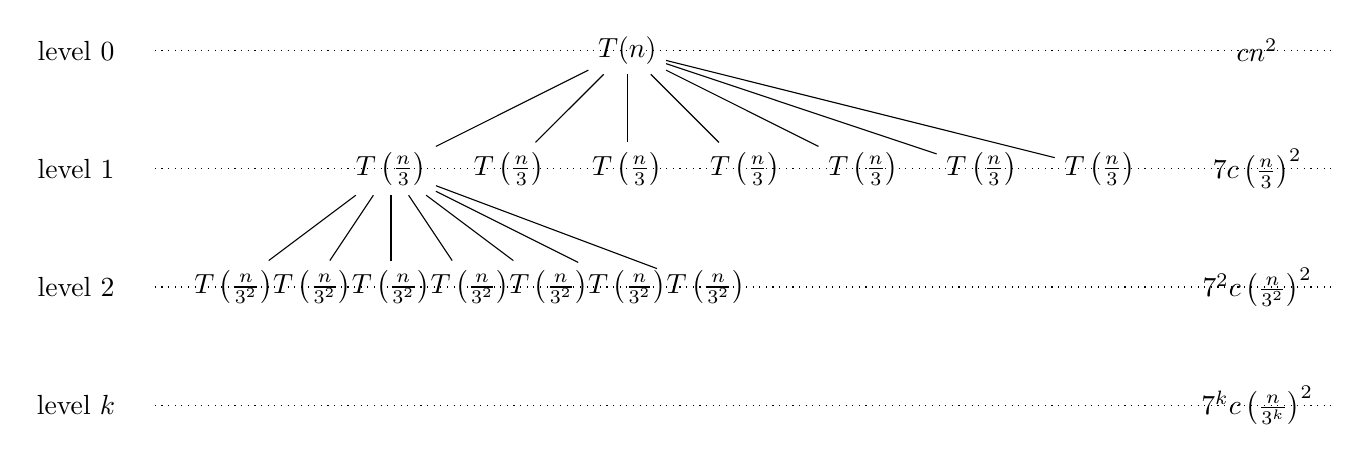
\begin{tikzpicture}
			% Nodes for level 0
			\node (Tn) at (0,0) {$T(n)$};
	
			% Nodes for level 1
			\node (Tn3-1) at (-3,-1.5) {$T\left(\frac{n}{3}\right)$};
			\node (Tn3-2) at (-1.5,-1.5) {$T\left(\frac{n}{3}\right)$};
			\node (Tn3-3) at (0,-1.5) {$T\left(\frac{n}{3}\right)$};
			\node (Tn3-4) at (1.5,-1.5) {$T\left(\frac{n}{3}\right)$};
			\node (Tn3-5) at (3,-1.5) {$T\left(\frac{n}{3}\right)$};
			\node (Tn3-6) at (4.5,-1.5) {$T\left(\frac{n}{3}\right)$};
			\node (Tn3-7) at (6,-1.5) {$T\left(\frac{n}{3}\right)$};
	
			% Nodes for level 2 (only showing first branch for brevity)
			\node (Tn9-1) at (-5,-3) {$T\left(\frac{n}{3^2}\right)$};
			\node (Tn9-2) at (-4,-3) {$T\left(\frac{n}{3^2}\right)$};
			\node (Tn9-3) at (-3,-3) {$T\left(\frac{n}{3^2}\right)$};
			\node (Tn9-4) at (-2,-3) {$T\left(\frac{n}{3^2}\right)$};
			\node (Tn9-5) at (-1,-3) {$T\left(\frac{n}{3^2}\right)$};
			\node (Tn9-6) at (0,-3) {$T\left(\frac{n}{3^2}\right)$};
			\node (Tn9-7) at (1,-3) {$T\left(\frac{n}{3^2}\right)$};
	
			% Edges for level 0 to level 1
			\draw (Tn) -- (Tn3-1);
			\draw (Tn) -- (Tn3-2);
			\draw (Tn) -- (Tn3-3);
			\draw (Tn) -- (Tn3-4);
			\draw (Tn) -- (Tn3-5);
			\draw (Tn) -- (Tn3-6);
			\draw (Tn) -- (Tn3-7);
	
			% Edges for level 1 to level 2 (first branch only)
			\draw (Tn3-1) -- (Tn9-1);
			\draw (Tn3-1) -- (Tn9-2);
			\draw (Tn3-1) -- (Tn9-3);
			\draw (Tn3-1) -- (Tn9-4);
			\draw (Tn3-1) -- (Tn9-5);
			\draw (Tn3-1) -- (Tn9-6);
			\draw (Tn3-1) -- (Tn9-7);
	
			% Cost Function Annotations
			\node at (8,0) {$cn^2$};
			\node at (8,-1.5) {$7c\left(\frac{n}{3}\right)^2$};
			\node at (8,-3) {$7^2c\left(\frac{n}{3^2}\right)^2$};
			\node at (8,-4.5) {$7^k c\left(\frac{n}{3^k}\right)^2$};
	
			% Levels
			\draw[dotted] (-6,0) -- (9,0);
			\draw[dotted] (-6,-1.5) -- (9,-1.5);
			\draw[dotted] (-6,-3) -- (9,-3);
			\draw[dotted] (-6,-4.5) -- (9,-4.5);
	
			\node at (-7,0) {level 0};
			\node at (-7,-1.5) {level 1};
			\node at (-7,-3) {level 2};
			\node at (-7,-4.5) {level $k$};
		\end{tikzpicture}
		\caption{Recurrence tree for $T(n) = 7T(n/3) + n^2$}
	\end{figure}
	\begin{itemize}
		\item Since we reduce the size by a factor of three each time, there are totally \( k = \log_3n\) levels. Summing all this up, we get:
		\begin{align}
			T(n) &= cn^2 + 7c\left(\frac{n}{3}\right)^2 + 7^2c\left(\frac{n}{3^2}\right)^2 + 7^3c\left(\frac{n}{3^3}\right)^2 + \ldots + 7^kc\left(\frac{n}{3^k}\right)^2 \label{eq:initial_sum} \\
				 &=  cn^2 \left( 7^0 \left(\frac{1}{3^0}\right)^2 + 7^1 \left(\frac{1}{3}\right)^2 +  7^2 \left(\frac{1}{3^2}\right)^2 + 7^3 \left(\frac{1}{3^3}\right)^2 + ... + 7^k \left(\frac{1}{3^k}\right)^2 \right) \\
				 &=  cn^2 \left( 7^0 \left(\frac{1}{3^2}\right)^0 + 7 \left(\frac{1}{3^2}\right) +  7^2 \left(\frac{1}{3^2}\right)^2 + 7^3 \left(\frac{1}{3^2}\right)^3 + ... + 7^k \left(\frac{1}{3^2}\right)^k \right) \\
				 &=  cn^2 \left( 1 + \left(\frac{7}{9}\right) +  \left(\frac{7}{9}\right)^2 + \left(\frac{7}{9}\right)^3 + \ldots + \left(\frac{7}{9}\right)^k \right) \\
				 &= cn^2 \left( \sum_{i = 0}^{\log_{3}n} \left(\frac{7}{9}\right)^i \right) \label{eq:sum_series}
		\end{align}
		\item When we apply the bound on the geometric series to \eqref{eq:sum_series} with \( r = \frac{7}{9} \), we get:
		\begin{align}
			T(n) &= cn^2 \left( \frac{1 - \left(\frac{7}{9}\right)^{\log_3n + 1}}{1 - \frac{7}{9}} \right) \\
				 &= cn^2 \left( \frac{9}{2} \left( 1 - \left(\frac{7}{9}\right)^{\log_3n + 1} \right) \right) \\
				 &= cn^2 \left( \frac{9}{2} - \frac{9}{2} \cdot \frac{7}{9} \cdot \left(\frac{7}{9}\right)^{\log_3n} \right) \\
				 &=  cn^2 \left( \frac{9}{2} - \frac{7}{2} \cdot \left(\frac{7}{9}\right)^{\log_3n} \right)
		\end{align}
		\item Using the formula \( a^{\log_3b} = b^{\log_3a} \), we have:
		\begin{align*}
			T(n) &=  cn^2 \left( \frac{9}{2} - \frac{7}{2} \cdot \left(n\right)^{\log_3\frac{7}{9}} \right) \\
				 &= cn^2 \left( \frac{9}{2} - \frac{7}{2} \cdot \left(n\right)^{\log_3 7 - 2} \right) \\
				 &= cn^2 \left( \frac{9}{2} - \frac{7}{2} \cdot \left(\frac{n^{\log_3 7}}{n^2}\right) \right) \\
				 &= \frac{9}{2}cn^2 - \frac{7}{2}cn^2 \cdot \frac{n^{\log_3 7}}{n^2} \\
				 &= \frac{9}{2}cn^2 - \frac{7}{2}cn^{\log_3 7} \\
		\end{align*}
	\end{itemize}
	Since \(\log_3 7\) is a constant, the term \(\frac{7}{2}cn^{\log_3 7}\) is much smaller than \(\frac{9}{2}cn^2\), and we can conclude that \(T(n) = \Theta(n^{2})\).

	\subsection*{h) \(T(n) = T(\sqrt{n}) + \log n\)}
	\begin{tikzpicture}
		\node (Tn) at (0,0) {$T(n)$};
		\node (Tn2-1) at (0,-1.5) {$T\left(\sqrt{n}\right)$};
		\node (Tn4-1) at (0,-3) {$T\left(\sqrt[4]{n}\right)$};
		
		\draw (Tn) -- (Tn2-1);
		\draw (Tn2-1) -- (Tn4-1);

		
		% Cost Function Annotations
		\node at (8,0) {$c\log_2n$};
		\node at (8,-1.5) {$c\left(\log_2\sqrt{n}\right)$};
		\node at (8,-3) {$c\left(\log_2\sqrt[4]{n}\right)$};
		\node at (8,-4.5) {$c\left(log_2\sqrt[(2^k)]{n}\right)$};
		
		% Levels
		\draw[dotted] (-6,0) -- (7,0);
		\draw[dotted] (-6,-1.5) -- (7,-1.5);
		\draw[dotted] (-6,-3) -- (7,-3);
		\draw[dotted] (-6,-4.5) -- (7,-4.5);
		
		\node at (-7,0) {level 0};
		\node at (-7,-1.5) {level 1};
		\node at (-7,-3) {level 2};
		\node at (-7,-4.5) {level $k$};
	\end{tikzpicture}
	\begin{itemize}
		\item From \(T(n) = T(\sqrt{n}) + \log_2n\) we can also write as:
		\[T(n) = T(n^{1/2}) + \log_2n\]
		% \item Then by recurrence, we have:
		% \begin{align}
		% 	T(n^{1/2}) &= T(n^{1/4}) + \log_2(n^{1/2}) \\
		% 	T(n^{1/4}) &= T(n^{1/8}) + \log_2(n^{1/4}) \\
		% 	&\ldots\\
		% 	T\left(n^{(2^{-m})}\right) &= T\left(n^{\left(2^{-(m + 1)}\right)}\right) + log_2(n^{(2^{-m})})
		% \end{align}
		\item This does not show a constant where we can stop. Therefore we need to subtitute n (Let \(n = 2^m\)), we have:
		\begin{align}
			T(2^m) &= T(2^{m/2}) + \log_2(2^m) \\
		           &= T(2^{m/2}) + m \Comment{Using Power rule} \\
		\end{align}
		\item Let \(S(m) = T(2^m)\) so \(S(m/2) = T(2^{m/2})\). Thus, we have:
		\begin{align}
			S(m) = S(m/2) + m \label{1:8:1}
		\end{align}
		\item Now we will find the complexity of \eqref{1:8:1}
		\begin{itemize}
			\item Since we halve the size everytime, there are totally \(k = \log_2m\) levels. Summing all this up,we get:
			\begin{align}
				S(m) &= c(\frac{m}{2^0}) + c(\frac{m}{2}) + c(\frac{m}{2^2}) + ... + c(\frac{m}{2^k}) \\
				     &= cm\left((\frac{1}{2})^0 + (\frac{1}{2})^1 + (\frac{1}{2})^2 + ... + (\frac{1}{2})^k\right) \label{1:8:2}
			\end{align}
			\item When we apply the bound on the geometric series to \eqref{1:8:2} with \( r = \frac{1f}{2} \), we get:
			\begin{align}
				S(m) &= cm\left(\frac{(\frac{1}{2})^{k + 1} - 1}{\frac{1}{2} - 1}\right) \\
				     &= -2cm\left(\left(\frac{1}{2}\right)^{\log_2(m) + 1} - 1\right) \\
					 &= -2cm\left(\frac{1}{2}\left(\frac{1}{2}\right)^{\log_2m} - 1\right) \\
					 &= -2cm\left(\frac{1}{2}m^{\log_2(\frac{1}{2})} - 1\right) \\
					 &= -2cm\left(\frac{1}{2m} - 1\right) \\
					 &= -c + 2cm \\
			\end{align}
			\item \(2cm\) is a dominant term. Thus, the complexity of \(S(m) = \Theta(m)\)
		\end{itemize}
		\item We started with the recurrence \(T(n) = T(\sqrt{n}) + \log_2n\) and transformed n to \(2^m\), which led us to a new recurrence \(S(m) = S(m/2) + m\), where \(S(m) = T(2^m)\). At the same time, complexity of \(S(m) = \Theta(m)\) and \(m = \log_2n\), substituting back, we get:
		\[S(\log_2n) = \Theta(\log_2n)\]
		\item By our transformation definition \(S(m) = T(2^m)\). Setting \(m = \log_2n\) implies \(2^m = n\). Thus, we have:
		\[S(\log_2n) = T(n)\]
		\item Therefore, substituting our expression for \(\log_2n\):
		\[T(n) = \Theta(\log_2n)\]
	\end{itemize}

	\newpage \section*{Problem 2}
	\subsection*{2.1 Combine two top Skeleton as an input and produce single top Skeleton in \(O(n)\)}
	\begin{enumerate}[label=({\alph*})]
		\item \textbf{Description of algorithm:}
		\begin{enumerate}
			\item Firstly, we have two dynamic arrays, which are the top skeleton of the first top skeleton and second top skeletons\(H_1\) and \(H_2\). 
			\begin{itemize}
				\item I call \textbf{\(H_1\)} is the dynamic array store top skeleton in the first top skeleton, which being sorted by horizontal segments ordered from left to right
				\item I call \textbf{\(H_2\)} is the dynamic array store top skeleton in the second top skeletons, which being sorted by horizontal segments ordered from left to right
			\end{itemize}
			\item Thus, when I access each segment in both top skeletons, it will cost \(\Theta(1)\) time, and each segment in both \textbf{\(H_1\)} and \textbf{\(H_2\)} is the array of size three with the first and second elements are left and right x-coordinates of the segment respectively and the third element denotes the y-coordinate of that segment.
			\item With the example of the image belows we will have the following input
			\begin{figure}[h]
				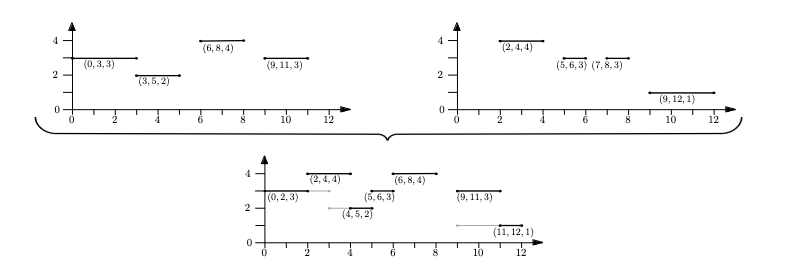
\includegraphics[width=16cm]{example2.png}
			\end{figure}
			\begin{itemize}
				\item In this example, we will have inputs:
				\begin{align}
					H_1 &= \{\{0, 3, 3\}, \{3, 5, 2\}, \{6, 8, 4\}, \{9, 11, 3\}\} \\
					H_2 &= \{\{2, 4, 4\}, \{5, 6, 3\}, \{7, 8, 3\}, \{9, 12, 3\}\}
				\end{align}
				\item And the expected output will be an dynamic array calls \textbf{result}. Thus, each time we add new element in that dynamic array will have the complexity is \(\mathcal{O}(1)\) amortized time.
				\item For this example, the output will be
				\begin{align}
					result &= \{\{0, 2, 3\}, \{2, 4, 4\}, \{4, 5, 2\}, \{5,6,3\}, \{6, 8, 4\}, \{9, 11, 3\}, \{11, 12, 1\}\}
				\end{align}
			\end{itemize}
			\item The pseudocode of function \verb|CombineSkeletons(H1, H2)|, after having the pseudocode I will explain how it works. Before writting the pseudocode I will have some function, which I will use in the pseudocode
			\begin{itemize}
				\item \verb|min(a, b)|: return the minimum value of integer a and integer b (The complexity is \(O(1)\))
				\item \verb|max(a, b)|: return the maximum value of integer a and integer b (The complexity is \(O(1)\))
				\item \verb|append(segment)|: append a segment into dynamic array. Because I use dynamic array to store and append always import new element at the end of the list so the complexity will be \(O(1)\)
			\end{itemize}
			\begin{algorithm}[H]
		\caption{CombineSkeletons}
	\begin{algorithmic}[1]
		\Function{CombineSkeletons}{\(H_1\), \(H_2\)}
		\State H = [] \Comment{Final TopSkeletons}
    	\State i, j = 0, 0 \Comment{Shift indices for H1 and H2}
		\While{i \(<\) length of \(H_1\) and j \(<\) length of \(H_2\)}
			\State \(\verb|Array|\) segment\_1 \(\leftarrow\) \(H_1[i]\)
			\State \(\verb|Array|\) segment\_2 \(\leftarrow\) \(H_2[j]\) \Comment{Comparing two segments from \(H_1\) and \(H_2\) to solve collapse}
			\If{\(segment\_1[1] \geq segment\_2[0]\) and \(segment\_1[1] \geq segment\_2[0]\)} \Comment{case when collapsed}
				\State min\_start \(\leftarrow\) \textbf{min}(segment\_1[0], segment\_2[0])
				\State max\_start \(\leftarrow\) \textbf{max}(segment\_1[0], segment\_2[0])
				\State min\_end \(\leftarrow\) \textbf{min}(segment\_1[1], segment\_2[1])
				\State max\_end  \(\leftarrow\) \textbf{max}(segment\_1[1], segment\_2[1])
				\Comment{Find unique point two split two segments into three intervals, which are first, second and third part}

				\State first\_part \(\leftarrow\) []
				\State third\_part \(\leftarrow\) []
				\If{segment\_1[0] \(<\) segment\_2[0]} \Comment{Case for finding the height of first interval}
					\State first\_part \(\leftarrow\) [min\_start, max\_start, segment\_1[2]]
				\Else{}
					\State first\_part \(\leftarrow\) [min\_start, max\_start, segment\_2[2]]
				\EndIf{}
				\State second\_part \(\leftarrow\) [max\_start, min\_end, \textbf{max}(segment\_1[2], segment\_2[2])] \Comment{Second interval}
				\If{segment\_1[1] \(>\) segment\_2[1]} \Comment{Case for finding the height of third interval}
					\State third\_part \(\leftarrow\) [min\_end, max\_end, segment\_1[2]]
				\Else{}
					\State third\_part \(\leftarrow\) [min\_end, max\_end, segment\_2[2]]
				\EndIf{}

				\Comment{After having three different interval, now I will check that the case two segments will have the that interval or not, if not starting x-cor and ending x-cor will be the same}
				\If{first\_part[0] != first\_part[1]} \Comment{If we exist the first\_part, add it to final dynamic array}
					\State H.\textbf{append}(first\_part)
				\EndIf{}
				\If{second\_part[0] != second\_part[1]} \Comment{If we exist the second\_part, add it to final dynamic array}
					\State H.\textbf{append}(second\_part)
				\EndIf{}

				\Comment{Now we will check the last part, which will need to add back to H\_1 or H\_2}
				
				\If{segment\_1[1] \(>\)segment\_2[1]} \Comment{segment\_1 extends beyond the end of segment\_2, which means the third part will be back in H\_1}
					\If{third\_part[0] != third\_part[1]} \Comment{check the existance of third part}
						\State H\_1[i] = third\_part
					\EndIf{}
					\State j \(\leftarrow j + 1\)
				\ElsIf{segment\_1[1] \(<\)segment\_2[1]} \Comment{the third part will be in H\_2}
					\If{third\_part[0] != third\_part[1]} \Comment{check the existance of third part}
						\State H\_1[i] = third\_part
					\EndIf{}
					\State i \(\leftarrow i  + 1\)
				\Else{} \Comment{The case that they have same endpoint, thus we will skip to next index in both array}
					\State j \(\leftarrow j + 1\)
					\State i \(\leftarrow i  + 1\)
				\EndIf{}
			\Else{} \Comment{If they are not collapse, find correct segment and put it into H}
				\If{segment\_1[0] \(<\) segment\_2[0] or (segment\_1[0] \(==\) segment\_2[0] and segment\_1[1] \(\leq\) segment\_2[1])} \Comment{This case, segment1 will be appended to H}
					\State H.\textbf{append}(segment\_1)
					\State i \(\leftarrow\) i + 1
				\Else
					\State H.\textbf{append}(segment\_2)
					\State j \(\leftarrow\) j + 1
				\EndIf
			\EndIf{}
		\EndWhile{}
		\While{i \(<\) \textbf{length}(H\_1)} \Comment{Add remaining segments}
        	\State H.\textbf{append}(H\_1[i])
        	\State i \(\leftarrow\) i + 1
    	\EndWhile{}
    	\While{j \(<\) \textbf{length}(H\_2)}
        	\State H.\textbf{append}(H\_2[j])
        	\State j \(\leftarrow\) j + 1
    	\EndWhile{}
		\State \Return{H}
		\EndFunction{}
	\end{algorithmic}
	\end{algorithm}
		\item As in the example, the output of the \verb|CombineSkeletons| is
		\[H = \{\{0, 2, 3\}, \{2, 3, 4\}, \{3, 4, 4\}, \{4, 5, 2\}, \{5, 6, 3\}, \{6, 7, 4\}, \{7, 8, 4\}, \{9, 11, 3\}, \{11, 12, 1\}\}\]
		\item As we can see this output is correct with H is a top Skeleton. However, some segments can be merged with other segments. Thus, to make the output shorter like the output of template, I will have another methods, which calls \verb|merging(H)| run in \(O(n)\) time
		\begin{algorithm}[H]
			\caption{Merging algorithm}
		\begin{algorithmic}[1]
			\Function{merging}{H}
			\State result \(\gets\) []
			\For{each segment $\textit{seg}$ in $H$}
				\If{$\textit{merged\_H}$ is not empty \AND last element in $\textit{merged\_H}$ ends at the same point where $\textit{seg}$ starts \AND last element in $\textit{merged\_H}$ has the same height as $\textit{seg}$}
					\State Update the end point of the last segment in $\textit{merged\_H}$ to the end point of $\textit{seg}$
				\Else{}
					\State Add $\textit{seg}$ to $\textit{merged\_H}$
				\EndIf{}
			\EndFor{}
			\State Return $\textit{merged\_H}$
			\EndFunction{}
		\end{algorithmic}
		\end{algorithm}
		\item using \verb|merging| function I will have expected output, which is
		\[H = \{\{0, 2, 3\}, \{2, 4, 4\}, \{4, 5, 2\}, \{5, 6, 3\}, \{6, 8, 4\}, \{9, 11, 3\}, \{11, 12, 1\}\}\]
		\item \textbf{Description how my algorithms works}
		\begin{itemize}
			\item Firstly, I will initialise a new dynamic array to store the result of combining two topSkeletons (final merged segments) and I Initialize indices \(i\) and \(j\) to 0. These will iterate \(H_1\) and \(H_2\) respectively.
			\item After that, I will have the main loop, and there loop will continue looping as long as there are segments left in both \(H_1\) and \(H_2\). In the loop, I Retrieve the current segments from \(H_1\) and \(H_2\) using indices i and j. Then, I will check the segments are overlap or not. This is done by checking  if the end of one segment is greater than or equal to the start of the other and vice versa.
			\begin{itemize}
				\item \textbf{Case 1: Two segments does not overlap} \Comment{It will go to first else confition in Pseudocode of CombineSkeleton}
				\begin{itemize}
					\item \textbf{Segment from $H_2$ extends beyond $H_1$}: Append $segment\_1$ to $H$ and increase the indices i for H\_1 by 1.
        			\item \textbf{Segment from $H_1$ extends beyond $H_2$}: Append $segment\_2$ to $H$ and  increase the indices i for H\_2 by 1.
				\end{itemize}
				\item \textbf{Case 2: Two segments overlaps} \Comment{It will go to the first if condition in Pseudocode}
				\begin{itemize}
					\item When segments s1 and s2 overlap, the algorithm will divide the segment into thre parts, which calls first\_part, second\_part and third\_part. Thus, to splits into three parts, I have to find significant points using \verb|min| and \verb|max| functions \Comment{From line 8 to 11 in Pseudocode}
					\begin{itemize}
						\item \verb|min_start|: the left-most point of the overlap
						\item \verb|max_start|: the second left-most point of the ovdrlap
						\item \verb|min_end|: the third left-most point of the overlap
						\item \verb|max_end|: the right-most point of the overlap
					\end{itemize}
					\item From all significant points of the overlap, I will have three part. \Comment{from line 12 to line 22 in Pseudocode}
					\begin{itemize}
						\item \verb|first_part|: will be the array of size 3, which is \{\verb|min_start|, \verb|max_start|, \textbf{y-coordinate of the segment that have min\_start}\}
						\item \verb|second_part|: will be the array of size 3, which is \{\verb|max_start|, \verb|min_end|, \textbf{y-coordianate of the segment that have max y-coordinate}\}
						\item \verb|third_part|: will be the array of size 3, which is \{\verb|min_end|, \verb|max_end|, \textbf{y-coordianate of the segment that have max\_end}\}
					\end{itemize}
					\item After we have three part, I will check \verb|first_part|: \Comment{From line 23 to 24 in Pseudocode}
					\begin{itemize}
						\item If the first part, if start point is the sam as end point, I will not add that part to H, because when they have the same start and end point, which means two segments at this case when overlap does not have first part. Otherwise, I will add \verb|first_part| to H
					\end{itemize}
					\item for the \verb|second_part|, I will do the same as I did for \verb|first_part| \Comment{from line 25 to 26 in Pseudocode}
					\item For the \verb|third_part|, I will do differently with the first two part \Comment{From line 27 to 37}
					\begin{itemize}
						\item First, I will use if condition to check which segment extends beyond the other segment. For example segment\_1 extends beyond segment\_2, I will change value of \(H_1\) at index i to the third part and increase j by 1. Other case like  segment\_2 extends beyond segment\_1, I will change value of \(H_2\) at index j to the third part and increas i by 1. At the case two of them are equals, which means we do not have third part. Thus, I increase both i and j by 1
					\end{itemize}
				\end{itemize}
			\end{itemize}
			\item Finally, I will have to while-loop for H\_1 and H\_2 to add remaining segments
			\item To make the result like expected output, I will call \verb|merging|.
			\begin{itemize}
				\item This function will create a new dynamic array calls result. 
				\item After that, it will start for-loop to terate over each segment "\(seg\)". In that loop, I will have condition for merging, which are;
				\begin{itemize}
					\item Check if the merged\_H list is not empty.
					\item Check if the end point of the last segment in \verb|merged_H|  is equal to the start point of the current segment
					\item Check if the height of the last segment in merge\_H s the same as the height of the current segment
				\end{itemize}
				\item \textbf{Merging segment}: If all the conditions are met, update the end point of the last segment in merged\_H to the end point of the current segment 
				\item \textbf{Adding New Segment}: If any of the conditions are not met, Add the current segment to merged\_H 
			\end{itemize}
		\end{itemize}
		\end{enumerate}
		\item \textbf{Argue the correctness}
		\begin{itemize}
			\item The algorithm correctness can be showed by utilizing loop invariant.
			\begin{itemize}
				\item \textbf{Invariant}: At the beginning of every iteration of the while loop, the list $H$ comprises the accurately processed segments considered thus far from both $H_1$ and $H_2$, with $H_1$ and $H_2$ being two top skeletons containing sorted segments.
				\item \textbf{Initialize}: At the start, before any iterations occur, the algorithm has not yet examined any segments from H\_1 and H\_2. As a result, H\_1 and H\_2 are unchanged, and H are empty. Therefore, the invariant is valid at this point. (It is important to note that both H\_1 and H\_2 are TopSkeletons)		
				\item \textbf{Maintenance}
				\begin{itemize}
					\item During each iteration, the algorithm will take the two segment at the value of H\_1 at index i and H\_2 at index j. After have that segments, the algorithm will have two cases, which is two segments are overlap or not by using conditional statement \Comment{The condition is in line 7}
					\item \textbf{Case 1: Overlap}
					\begin{itemize}
						\item After finding all the significant points, I will have three parts. With the first\_part that have starting coordinate at \verb|min_start| and end at \verb|end_start|. Thus, that part will node overlap with other segments. The reason for that is because it will end at the start of other segments.
						\item For the second\_part, it will starts at max\_start and end at min\_end. Thus, this part can be an overlap parts if this part exists. That is why the algorithm will remove the overlap part by choosing the part with higher y-coordinate. Not only that, because we choose only part with higher y-coordinate and skip append the part with lower coordinate, so after append this part to H, we do not have any overlap part in H. Thus, the invariant still holds 
						\item In term of the third\_part, because third\_part is the sub part of segment\_1 or segment\_2 depending on different cases, when we add back to H\_1 or H\_2 depending on the part is the sub part of segment\_1 and segment\_2. Thus, we do not have any overlap segments in H\_1 and H\_2 after add the third\_part back to index i or j. The reason for that is because before adding third\_part to H\_1 or H\_2, H\_1 and H\_2 are TopSkeletons, which means when I change that segment to sub part of that segment, H\_1 or H\_2 also be the TopSkeletons. Thus, the invariant still holds 
					\end{itemize}
					\item \textbf{Case 2: Not overlap}
					\begin{itemize}
						\item The algorithm picks the segment having ealier starting position element from two non-overlapping segments to include in set H
						H. This ensures that only correct segments are added to set H. Thus preserving the invariance.
					\end{itemize}
					\item After that, I will add every remaining segments of H\_1 or H\_2 into H. Because we have solved every overlap possible, all remaining segments is part of TopSkeletons. Thus, the loop invariant still holds
					\item  Taking all those into consideration, we can conclude that after each iteration, the invariant holds
				\end{itemize}
				\item \textbf{Termination}: The loop will terminate when we scan every segments in both H\_1 and H\_2 at least once. Thus, we will have H is the combine Top skeletons of H\_1 and H\_2. Thus, the invariant stills holds at termination
			\end{itemize}
			\item In conclusion, by maintaining the loop invariant in all iterations, the correctness of the algorithm is guaranteed.
		\end{itemize}
		\item \textbf{Prove an upper bound on the time complexity of your algorithm}:
		\begin{itemize}
			\item \textbf{Initialisation}: At the start, I initialise H equals to empty dynamic array. After that, I initialise i and j equals to 0. Thus, the complexity of this one is \(\mathcal{O}(1)\)
			\item \textbf{First While loop}: Let \(a\) is the size of H\_1 and \(b\) is the size of H\_2. The main while loop will have \(a + b\) iterations. Each iteration will run in \(\mathcal{O}(1)\) time, which being proved belows
			\begin{itemize}
				\item In each iteration, the algorithm will retrieve the current segments from \verb|H_1| and \verb|H_2| using indices i and j. Thus, the complexity of this one is \(\mathcal{O}(1)\) \Comment{in line 5 and 6}
				\item After that, I will have the first condtional statement to check two segments are overlap or not in \(O(1)\) time. \Comment{in line 7 of Pseudocode}
				\begin{itemize}
					\item If the condtion are true it will run in line 8 to line 37 in Pseudocode. From line 8 to line 13, all of this lines will run in O(1) time becasue it just merely assigning using \verb|min| and \verb|max| function, which is being proved run in O(1) time before. In line 14, 19, 23, 25, 27, 31 in Pseudocode, we will have seperate conditional statements, which run in \(\mathcal{O}(1)\) time. This is mainly because it just a logical operations. In each conditional statements, It run in \(\mathcal{O(1)}\) time because inside each conditional statements, It just increase i or j by 1 or using \verb|append| function or changing the value in H\_1 or H\_2 by using index. All of these will run in \(O(1)\) time. Thus inside in each iteration, it will run in constant time, which is \(\mathcal{O}(1)\)
					\item If the condition are not true, it will run in line 39 to 44. Because the condtion statement in line 39 run in \(O(1)\) and inside that conditional statement it also run in \(O(1)\) time (\verb|append| runs in O(1) time). Thus, in each iteration, it will run in \(O(1)\) time. 
				\end{itemize}
				\item After that, I will have two while loop which runs in \(O(a)\) and \(O(b)\). This is because in side them, the algorithm use only \verb|append| function and increase indicies by one. Thus both of them run in \(O(a)\) or \(O(b)\) time
			\end{itemize}
			\item The complexity of this algorithm is:
			\[O(1) + O(1) + O(a + b) + O(a) + O(b) = \mathcal{O}(a + b) = \mathcal{O}(n) \quad \blacksquare\] 
		\end{itemize}
	\end{enumerate}
	\subsection*{2.2: Divide-and-Conquer algorithm that computes the top skeleton of a set S of n horizontal line
	segments in the plane}
	\begin{enumerate}[label = \alph*]
		\item \textbf{Description how my algorithms works}
		\begin{algorithm}[H]
			\caption{Wrong algorithm}
		\begin{algorithmic}[1]
			\Function{TopSkeletons}{S}
			\If{Size of s larger than 1}
				\State mid \(\leftarrow \text{int}(\frac{\text{size of s}}{2})\) 
				\State top1 \(\leftarrow\) TopSkeletons(ls[:mid])
				\State top2 \(\leftarrow\) TopSkeletons(ls[mid:])
				\State \Return{CombineSkeleton(top1, top2)} 
			\Else{}
				\State \Return{S} 
			\EndIf{}
			\EndFunction{}
		\end{algorithmic}
		\end{algorithm}
		\begin{itemize}
			\item My algorithm uses Divide and Conquer, so I will explain it in two steps: dividing and conquering.
			
			\item \textbf{Dividing and Conquere}
			\begin{itemize}
				\item My algorithm uses recursion to divide the original skeletons until the size of the skeletons equals 1, which means the size of an input to the \texttt{TopSkeletons} function equals 1. First, I need a conditional statement to check if the size of the input is larger than 1 \Comment{Line 2 of the pseudocode}. If the size equals 1, I will stop the dividing step and return that array. If the size of the input is larger than 1, I will assign \texttt{mid} to half the number of segments in $S$, and use recursion to assign \texttt{top1} and \texttt{top2}.
			\end{itemize}	
			\item \textbf{Combining}
			\begin{itemize}
				\item After dividing the original skeletons into subproblems, the algorithm proceeds to combine the results. Once \texttt{top1} and \texttt{top2} are computed by recursively calling \texttt{TopSkeletons} on the divided segments, the \texttt{CombineSkeleton} function is called to merge these results \Comment{Line 5 of the pseudocode}. This function ensures that the combined skeleton maintains the properties required by the algorithm.
				\item The \texttt{CombineSkeleton} function takes \texttt{top1} and \texttt{top2} as inputs and merges them, ensuring that no incorrect segments are included in the combined result. The specifics of this merging process depend on the criteria defined by the problem, such as maintaining order or ensuring no overlaps.
				\item Finally, the combined skeleton is returned as the result of the \texttt{TopSkeletons} function call. By ensuring that each recursive step correctly processes and combines the segments, the algorithm maintains its correctness and efficiency.
			\end{itemize}
		\end{itemize}
		Overall, this Divide and Conquer approach effectively breaks down the problem into smaller, manageable parts, solves each part recursively, and then combines the results to form the final solution.
		\item \textbf{Argue the correctness}
		\begin{itemize}
			\item We prove this algorithm's correctness via induction
			\item Base case: when the input has 1 or 0 segment, that input is trivially the top skeleton of itself sorted from left to right, returning the correct result.
			\item Recursive case: If we have calculated the top skeletons of the two halves correctly, we can find the top skeletons sorted from left to right of both halves combined correctly. This is ensured by the correctness of our CombineSkeletons() algorithm.
			\item Addendum: the program always reaches its base case as by dividing the input list in half repeatedly, we will always reach the base case where the original list has been divided into lists with less than 2 segments within.
			\item As the base case is correct and the recursive case maintains this correctness, we can conclude that this algorithm is correct.
		\end{itemize}
		\item \textbf{Analysis the complexity}
		\begin{itemize}
			\item In the base case, the algorithm simply returns the list itself, which takes \( O(1) \) time. The divide step also runs in \( O(1) \) time because it only involves calculating the midpoint and slicing the original list. The recursive step computes the top skeleton for each half recursively, and the combine step takes \( O(n) \) time for \( n \) segments. Thus, we have the following recurrence relation:
			\[
				T(n) =
				\begin{cases} 
					T(n) = 2T(n/2) + O(n) & \text{for } n > 1 \\
					O(1) & \text{for } n \leq 1 
				\end{cases}
			\]
		\end{itemize}
		\item Thus, I will have the following chart then I will prove using unrolling
		\item Since we halve the size every time. Thus, the level is \(k = \log_2n\). Summing all this up, we get
	\end{enumerate}
	\begin{tikzpicture}
		\node (Tn) at (0,0) {$T(n)$};
		\node (Tn2-1) at (-3,-1.5) {$T\left(\frac{n}{2}\right)$};
		\node (Tn2-2) at (3,-1.5) {$T\left(\frac{n}{2}\right)$};
		\node (Tn4-1) at (-5,-3) {$T\left(\frac{n}{2^2}\right)$};
		\node (Tn4-2) at (0,-3) {$T\left(\frac{n}{2^2}\right)$};
		
		\draw (Tn) -- (Tn2-1);
		\draw (Tn) -- (Tn2-2);
		\draw (Tn2-1) -- (Tn4-1);
		\draw (Tn2-1) -- (Tn4-2);
		\draw (Tn2-2) -- (3, -3);
		\draw (Tn2-2) -- (6, -3);


		
		% Cost Function Annotations
		\node at (8,0) {$c\cdot n \cdot$};
		\node at (8,-1.5) {$2c\cdot \frac{n}{2}$};
		\node at (8,-3) {$2^2c\cdot \frac{n}{2^2}$};
		\node at (8,-4.5) {$2^kc\cdot \frac{n}{2^k}$};
		
		% Levels
		\draw[dotted] (-6,0) -- (7,0);
		\draw[dotted] (-6,-1.5) -- (7,-1.5);
		\draw[dotted] (-6,-3) -- (7,-3);
		\draw[dotted] (-6,-4.5) -- (7,-4.5);
		
		\node at (-7,0) {level 0};
		\node at (-7,-1.5) {level 1};
		\node at (-7,-3) {level 2};
		\node at (-7,-4.5) {level $k$};
	\end{tikzpicture}
	\begin{align}
		T(n) &= cn + 2c\frac{n}{2} + 2^2c\frac{n}{2^2} + ... + 2^kc\frac{n}{2^k} \\
		     &= cn\left((\frac{2}{2})^0 + (\frac{2}{2})^1 + (\frac{2}{2})^2 + ... + (\frac{2}{2})^k\right) \\
			 &= cn\left(1^0 + 1^1 + 1^2 + ... + 1^k\right) \\
	\end{align}
	Because k = \(\log_2n\), \(\left(1^0 + 1^1 + 1^2 + ... + 1^k\right) = \log_2n\)
	
	Thus, we have:
	\[T(n) = 2\log_2n\]
	Thus, the complexity of the algorithm is \(\mathcal{O}(n\log_2n)\)
\end{document}